\documentclass[12pt,a4paper,titlepage]{article}
\usepackage[utf8]{inputenc}

\usepackage[left=1.5cm,right=2cm,top=2cm,bottom=2cm]{geometry}
\usepackage{amsmath}
\usepackage{amssymb}
\usepackage{amsthm}
\usepackage{hyperref}
\usepackage{graphicx}
\usepackage[space]{grffile}

\usepackage{listings}
\lstset{language=Java}


\newcommand{\class}[1]{\texttt{#1}}

\author{Jonathan Visbecq, Gaspard Férey}
\title{Projet d'INF 431 \\ - \\ Rapport}


\begin{document}
\maketitle

\section*{Introduction}

\section*{Classes annexes}

\subsection*{La lecture des fichiers}

\begin{figure}
	\label{fig:fileManagerPackage}
	\centering
	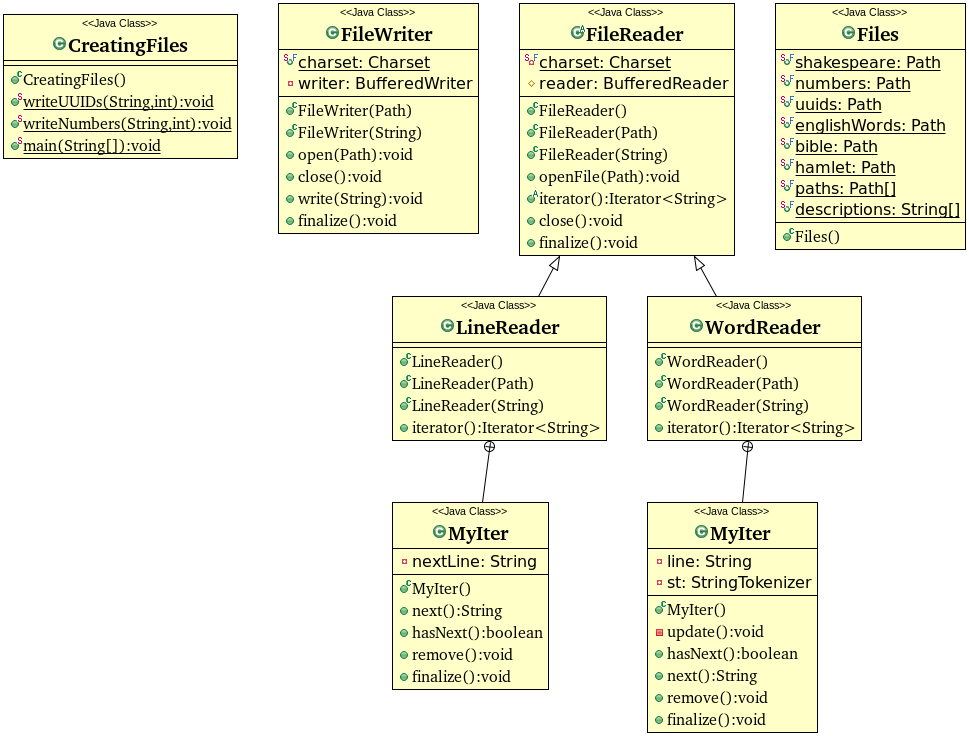
\includegraphics[scale=0.65, angle=90]{../Java Workspace/Test Hash/fileManagerPackage.png}
	\caption{Le package fileManagerPackage.}
\end{figure}

Le traitement du sujet suggère la manipulation fréquente de gros fichiers textes.\\
Les classes du package \class{FileManager} permettent de faciliter l'utilisation des fichiers. Par exemple, elles permettent de les désigner par leur chemin \class{Path} ou leur adresse \class{String} et gèrent les éventuelles exceptions lors du traitement en interne. En particulier, on y trouve :
\begin{itemize}
\item La classe abstraite \class{FileReader} qui permet d'ouvrir en lecture un fichier.\\
	Cette classe implémente l'interface \class{Iterable<String>} et permet donc de parcourir le fichier à l'aide d'une simple boucle \class{for}.
	Elle possède deux classes filles :
	\begin{itemize}
	\item La classe \class{WordReader} qui permet de lire un fichier mot à mot.
	\item La classe \class{LineReader} qui permet de lire un fichier ligne à ligne.
	\end{itemize}
\item La classe \class{FileWriter} qui permet l'écriture dans un fichier.
\item La classe \class{Files} qui est simplement un catalogue des fichiers souvent utilisés.
\item La classe \class{CreatingFiles} qui contient des fonctions qui permettent des générer des fichiers volumineux de test. En particulier, ils permettent de génèrer :
	\begin{itemize}
	\item Un fichier des nombres de $0$ à $n$.
	\item Un fichier de $n$ identifiants UID générés pas Java.
	\end{itemize}
\end{itemize}

\subsection*{L'arithmétique en Java}
La classe \class{UnsignedArithmetic} du package \class{drafts} fournit des fonctions qui permettent la correcte implantation des opérateurs addition et soustraction de deux \class{int}. En effet, Java utilise une implantation interne du type \class{int} qui tend à préserver le bit de signe (bit de poids le plus fort) lors de certaines opérations.

\subsection*{Communiquer}
La classe \class{Draft} du package \class{drafts} fournit, elle, des fonctions utiles à l'interface avec l'utilisateur. En particulier elle contient des méthodes d'affichage et d'utilisation de la console.




\newpage
\section{Le hachage}

\begin{figure}
	\label{fig:hashPackage}
	\centering
	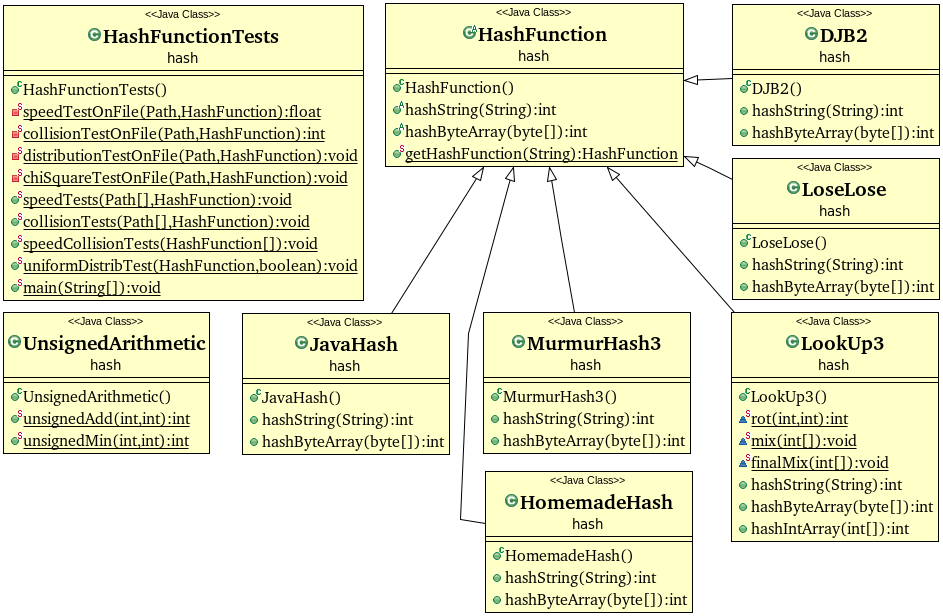
\includegraphics[scale=0.75, angle=90]{../Java Workspace/Test Hash/hashPackage.png}
	\caption{Le package \class{hash}.}
\end{figure}

Nous avons choisit de définir chacune des fonctions de hachage comme des sous-classes de la classe abstraite \class{HashFunction}.
Ainsi cette classe impose la définition des méthodes suivantes :
\begin{lstlisting}
	public int hashByteArray(byte[] array);
	public int hashString(String s);
\end{lstlisting}
dont l'implémentation dépends, bien sur, de la fonction de hachage et qui implémentent le hachage des types de données qui nous intéressent.

\subsection{Le hachage \class{LookUp3}}
Cette classe implante un hachage tel qu'il est décrit à adresse \href{http://www.burtleburtle.net/bob/c/lookup3.c}{cette adresse}.

\subsection{Le hachage \class{MurmurHash3}}
Cette classe implante un hachage tel qu'il est décrit à adresse \href{http://en.wikipedia.org/wiki/MurmurHash}{cette adresse}.

\subsection{Autres hachages}
Principalement pour les comparer aux deux précédents, nous avons définit d'autres fonctions de hachage :
\begin{itemize}
\item \class{DJB2} dont la description peut être trouvée à \href{http://www.cse.yorku.ca/~oz/hash.html}{cette adresse}.
\item \class{JavaHash}, la fonction de hachage par défaut de Java.
\item \class{LoseLose}, dont la description peut être trouvée à \href{http://www.cse.yorku.ca/~oz/hash.html}{cette adresse}.
\item \class{HomemadeHash} % au fait elle fait quoi cette fonction ?
\end{itemize}

\subsection{La classe \class{HashFunctionTests}}
Cette classe regroupe les méthodes permettant de comparer et tester les différentes fonctions de hachages.
On y trouve en particulier les méthodes suivantes :
\begin{itemize}

\item \begin{lstlisting}
private static float speedTestOnFile(Path path, HashFunction func)
\end{lstlisting}
Cette fonction parcours le fichier désigné par \class{path} et applique la fonction de hachage \class{func} sur chacun de ses mots. Elle retourne le temps que ce parcours a nécessité (en secondes).

\item \begin{lstlisting}
public static void speedTests(Path[] paths, HashFunction func)
\end{lstlisting}
Cette fonction effectue le même test sur tout les fichiers de \class{paths} et affiche les résultats dans la sortie standard.

\item \begin{lstlisting}
private static int collisionTestOnFile(Path path, HashFunction func)
\end{lstlisting}

\item \begin{lstlisting}
public static void collisionTests(Path[] paths, HashFunction func)
\end{lstlisting}
Cette fonction effectue le même test sur tout les fichiers de \class{paths} et affiche les résultats dans la sortie standard.

\item \begin{lstlisting}
private static void distributionTestOnFile(Path path, HashFunction func)
\end{lstlisting}

\item \begin{lstlisting}
private static void chiSquareTestOnFile(Path path, HashFunction func)
\end{lstlisting}

\end{itemize}



\newpage
\section{L'algorithme HyperLogLog}
La classe \class{HyperLogLog} contient les fonctions traitant la partie 2 du projet.\\

Les valeurs de $\alpha$ sont tabulées dans 
\begin{lstlisting}
static double[] alpha = { 0, 0.351194, 0.532435, 0.625609, ... };
\end{lstlisting}
Remarque : \class{alpha[b]} correspond à $\alpha_m$ avec $m=2^b$.\\

La fonction $\rho$ est déjà implantée en Java dans le package \class{Integer} ou elle porte le nom de \class{numberOfTrailingZeros}.
Nous fournissons également notre propre implantation :
\begin{lstlisting}
public static int rho(long x)
\end{lstlisting}

La fonction demandée en question 2 étant un cas particulier de la question 5), on décrira directement l'algorithme de la question 5), étant entendu qu'il est utilisé question 1) en prenant le paramètre $k$ égal à 1.

\subsection{Construction du tableau $M$}
Cette construction est implantée par la fonction suivante
\begin{lstlisting}
public static int[] buildFingerPrint(Path path, HashFunction func,
		int b, int k)
\end{lstlisting}
L'algorithme employé est celui décrit dans l'énoncé auquel sont apportées les modifications recommandées dans l'article de Flajolet \textit{et alii}.
En particulier les valeurs de $M$ sont initialisées à $0$ :
\begin{lstlisting}
int[] M = new int[m]; // M initialized to 0 by default
\end{lstlisting}

Pour traiter un $n$-uplet de mots, on conserve au cours de la lecture du fichier les $n$ dernier mots lus ainsi que leur taille.
Les mots sont ajoutés par
\begin{lstlisting}
strBuilder.append(s);
indexes.add(s.length());
\end{lstlisting}
et retirés par
\begin{lstlisting}
strBuilder.replace(0, indexes.poll(), "");
\end{lstlisting}



\subsection{Estimation du nombre de $k$-shingles distincts}
Le tableau $M$ construit précédemment est ensuite utilisé pour estimer le résultat selon l'algorithme spécifié dans l'énoncé. Cette estimation est stockée dans une variable \class{e}. On effectue ensuite le code suivant qui applique les modifications suggérées par l'article de Flajolet \textit{et alii}.
\begin{lstlisting}
if (e < 2.5 * m) {
    double v = 0;
    for (int i = 0; i < m; i++)
    	if (M[i] == 0) v++;
    if (v != 0)
    	e = m * Math.log(m / v);
} else if (e > n / 30)
    e = -n * Math.log(1 - e / n);
\end{lstlisting}
où $n = 2^{32}$.



\newpage
\section{Similarités entre ensembles de données}
Une instance de la classe \class{Similarities} permet de comparer deux à deux les fichiers fournit lors de sa création. L'initialisation consiste à créer les tableaux $M_i$ associés aux différents fichiers. Puis l'algorithme proposé dans l'énoncé est utilisé pour calculer $r(A,B)$ à travers la fonction
\begin{lstlisting}
private static double calculateResemblance(int[] MA, int[] MB, int b)
\end{lstlisting}
Cette fonction appliquée à toute les paires de fichiers permet de comparer leur ressemblance.


\newpage
\section{Fenêtre glissante}
On note $W$ la taille de la fenêtre.\\
L'enjeu de cet algorithme consiste à retenir à chaque instant du parcours du fichier la valeur maximale de \class{M[i]} (pour tout $i$) rencontrée lors des $W$ derniers mots. Pour cela on ne décrit pas $M$ pas un tableau d'entiers mais pas deux tableaux de listes de type \class{LinkedList<Integer>} qui sauvegardent respectivement:\\
\begin{tabular}{lcl}
\class{timestamps} &:& une valeur de $\rho$ rencontrée \\
\class{values} 	   &:& la date de la rencontre
\end{tabular}
Ceci nécessite de tenir un compteur de la date de lecture des mots.

\subsection{Insertion d'un élément}
Lors de l'insertion d'un élément $\rho$ à l'indice $i$ du tableau au temps \class{timestamp}, on consulte les deux listes $\class{values}_i$ et $\class{timestamps}_i$ :
\begin{lstlisting}
    while ( !values.isEmpty() && rho >= values.getFirst() ) {
    	values.remove();
    	timestamps.remove();
    }
    timestamps.addFirst(timestamp);
	values.addFirst(rho);
\end{lstlisting}
Ainsi on supprime tout les $\rho'$ lu précédemment qui sont inférieurs à $\rho$. En effet, ceux-ci n'ont plus aucune chance d'être le maximum de $M$ car un éléments plus grand vient d'arriver (est plus jeune dont sera supprimé après eux).
Ainsi cette insertion préserve plusieurs invariants :
\begin{itemize}
\item \class{values} et \class{timestamps} ont la même taille.
\item \class{values} est classée par ordre croissant.
\item \class{timestamps} est classé par ordre décroissant.\\
Car les \textit{timestamps} sont insérés successivement au cours de l'exécution, donc dans l'ordre croissant.
\end{itemize}

\begin{figure}[!h]
	\centering
	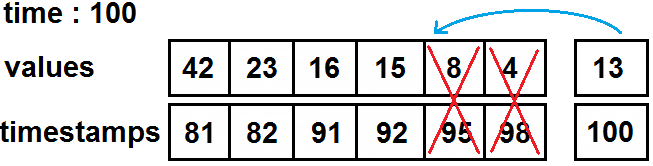
\includegraphics[scale=0.5]{pictures/picSlidingWindow2.png}
	\caption{Insertion d'un élément.}
\end{figure}

\newpage
\subsection{Nettoyage des listes}
A chaque utilisation des listes pour calculer \class{M[i]}, il faut s'assurer que le maximum a bien été suffisamment tôt. On supprime donc tout les couples (\class{timestamp}, \class{value}) qui sont plus vieux que la taille $W$ de la fenêtre. Le maximum est alors l'élément le plus vieux de la liste.

\begin{figure}[!h]
	\centering
	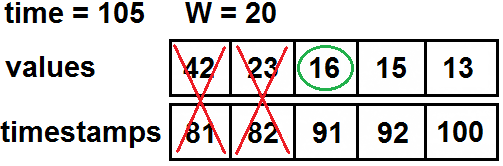
\includegraphics[scale=0.5]{pictures/picSlidingWindow1.png}
	\caption{Nettoyage des listes.}
\end{figure}

\subsection{Complexité en temps}
On effectue un passage sur tout les $N$ mots du fichier.\\
On effectue $S$ évaluations du nombre de mots distincts. A chaque évaluation il faut vérifier que les $m$ cases du tableau $M$ sont nettoyées.\\
L'ensemble des nettoyages va supprimer environ $N$ mots au total.\\

On en conclut que la complexité en temps est de $\mathcal{O}(N + mS)$. La complexité en temps reste donc linéaire à condition de ne pas être trop exigeant sur $S$.\\
Pour une représentation graphique, $S=1000$ suffit largement.

\subsection{Complexité en espace}
Le tableau $M$ ne contient plus uniquement $m$ entiers mais $2m$ listes d'entiers.\\
Cependant, ces listes ne contiennent en tout que $W+2N/S$ entiers maximum.
Les entiers de \class{timestamps} sont codés sur $\mathcal{O}(\log(N))$ bits au pire (et en moyenne).
Ceux de \class{values} sont codés sur $\mathcal{O}( \log(\log(N)) )$ bits en moyenne.
La complexité en espace est donc de $\mathcal{O}(\frac{N\log(N)}{S})$.

\subsection{Alternative}
Une alternative est d'effectuer un nettoyage supplémentaire de \class{M[i]} à chaque ajout d'une entrée à cet indice. Ainsi, la différence d'âge entre les plus vieux et plus jeunes n'excède jamais $W$ et le tableau ne peut donc pas contenir plus de $2Wm$ entiers.\\
La complexité en espace passe à $\mathcal{O}(mW\log(N))$.\\
La complexité en temps passe à  $\mathcal{O}(WN + mS)$.\\

On remarque qu'il n'est plus possible de retenir uniquement $\mathcal{O}(\log \log N)$ bits à cause de la nécessité de retenir les \class{timestamps}.
Cependant, comme il n'est pas nécessaire de retenir la date exacte, mais seulement la date relativement à la  date actuelle, on pourrait envisager d'effectuer de temps en temps une remise à jour de la date. Par exemple, comme les ages des entrées ne sont pas censées excéder $W$, on pourrait, tout les temps multiples de $W$, diminuer toutes les dates (actuelle et stockées dans $M$) de $W$. Ainsi, la complexité en temps est augmentée de $2Wm\frac{N}{W}$ mais le nombre de bit d'un \class{timestamp} devient $\mathcal{O}(\log S)$..\\
La complexité en espace passe à $\mathcal{O}(mW (\log \log N + \log W)) =^{(1)} \mathcal{O}(\log \log N)$.\\
La complexité en temps passe à $\mathcal{O}((W+m)N + mS) =^{(1)} \mathcal{O}(N)$.\\
$^{(1)}$ : Si $S$, $W$, $m$ et $N$ sont des constantes.



\newpage
\section{Souris}






\newpage
\section{Icebergs}





\newpage
\section*{Conclusion}




\end{document}
